\begin{figure*}[htbp!]
  \centering
  \begin{subfigure}{0.5\textwidth}
  \includegraphics[width=\textwidth, clip, trim={0 1.25cm 1.25cm 0}]{binder/teeplots/20/surface-size=16+viz=site-reservation-at-ranks-heatmap+ext=}
  \end{subfigure}%
  \begin{subfigure}{0.5\textwidth}
  \includegraphics[width=\textwidth, clip, trim={1.25cm 1.25cm 0 0}]{binder/teeplots/20/plotter=size+surface-size=16+viz=site-reservation-at-ranks-heatmap+ext=}
  \end{subfigure}

\begin{subfigure}{\linewidth}
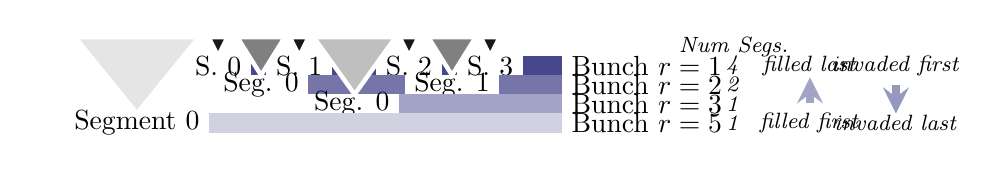
\begin{tikzpicture}[scale=\linewidth/50cm]
  % Define the total width and height

  % Create scope with normalized axes
  \begin{scope}
    % Grid
    % \draw[lightgray,step=1] (0,0) grid (50,4);

    % Axes' labels
    % \foreach \x in {1,5,...,49} { \node [below] at (\x,0) {\x}; }
    % \foreach \y in {0,1,...,4} { \node [left] at (0,\y) {\y}; }

% Add text
\node[anchor=west] (texta) at (27.0, 3.5) {Bunch $r=1$};
\node[anchor=west] (textb) at (27.0, 2.5) {Bunch $r=2$};
\node[anchor=west] (textc) at (27.0, 1.5) {Bunch $r=3$};
\node[anchor=west] (textd) at (27.0, 0.5) {Bunch $r=5$};

\node[anchor=center,font={\footnotesize}] (textx) at (36.0, 4.5) {\textit{Num Segs.}};
\node[anchor=center,font={\footnotesize}] (textax) at (36.0, 3.5) {\textit{4}};
\node[anchor=center,font={\footnotesize}] (textbx) at (36.0, 2.5) {\textit{2}};
\node[anchor=center,font={\footnotesize}] (textcx) at (36.0, 1.5) {\textit{1}};
\node[anchor=center,font={\footnotesize}] (textdx) at (36.0, 0.5) {\textit{1}};

\node[anchor=center,font={\footnotesize}] (textay) at (40.0, 3.5) {\textit{filled last}};
% \node[anchor=center] (textby) at (47, 2.5) {\textit{2}};
% \node[anchor=center] (textcy) at (47, 1.5) {\textit{1}};
\node[anchor=center,font={\footnotesize}] (textdy) at (40.0, 0.5) {\textit{filled first}};
\draw[-{stealth[scale=0.2]},shorten >=-1mm, shorten <=-0mm, line width=3pt,draw=MidnightBlue!40](textdy.north) -- (textay.south);

\node[anchor=center,font={\footnotesize}] (textay) at (44.5, 3.5) {\textit{invaded first}};
% \node[anchor=center] (textby) at (47, 2.5) {\textit{2}};
% \node[anchor=center] (textcy) at (47, 1.5) {\textit{1}};
\node[anchor=center,font={\footnotesize}] (textdy) at (44.5, 0.5) {\textit{invaded last}};
\draw[-{stealth[scale=0.2]},shorten >=-1mm, shorten <=-0mm, line width=3pt,draw=MidnightBlue!45](textay.south) -- (textdy.north);


% Triangles are drawn with the tip pointing downwards and base flush with y=5
\filldraw[draw=white,ultra thick,fill=black!90] (8.5,5) -- ++(0.5,-1) -- ++(0.5,1) -- cycle;
\node[anchor=center] (textaa) at (9, 3.5) {S.{} 0};
\filldraw[draw=white,ultra thick,fill=black!90] (12.75,5) -- ++(0.5,-1) -- ++(0.5,1) -- cycle;
\node[anchor=center] (textab) at (13.25, 3.5) {S.{} 1};
\filldraw[draw=white,ultra thick,fill=black!90] (18.5,5) -- ++(0.5,-1) -- ++(0.5,1) -- cycle;
\node[anchor=center] (textac) at (19, 3.5) {S.{} 2};
\filldraw[draw=white,ultra thick,fill=black!90] (22.75,5) -- ++(0.5,-1) -- ++(0.5,1) -- cycle;
\node[anchor=center] (textad) at (23.25, 3.5) {S.{} 3};

% \draw[-stealth, thick, draw=MidnightBlue!80](texta.east) -- (textaa.west);
% \draw[-stealth, thick, draw=MidnightBlue!80](textaa.east) -- (textab.west);
% \draw[-stealth, thick, draw=MidnightBlue!80](textab.east) -- (textac.west);
% \draw[-stealth, thick, draw=MidnightBlue!80](textac.east) -- (textad.west);
\draw[-, line width=7pt, draw=MidnightBlue!80](textaa.east) -- (textab.west);
\draw[-, line width=7pt, draw=MidnightBlue!80](textab.east) -- (textac.west);
\draw[-, line width=7pt, draw=MidnightBlue!80](textac.east) -- (textad.west);
\draw[-, line width=7pt, draw=MidnightBlue!80](textad.east) -- (texta.west);


% Add text
\filldraw[draw=white,ultra thick,fill=black!50] (10,5) -- ++(1.25,-2) -- ++(1.25,2) -- cycle;
\node[anchor=center] (textba) at (11.25, 2.5) {Seg.{} 0};
\filldraw[draw=white,ultra thick,fill=black!50] (20,5) -- ++(1.25,-2) -- ++(1.25,2) -- cycle;
\node[anchor=center] (textbb) at (21.25, 2.5) {Seg.{} 1};


% \draw[-stealth, thick,draw=MidnightBlue!60](textb.east) -- (textba.west);
% \draw[-stealth, thick,draw=MidnightBlue!60](textba.east) -- (textbb.west);
\draw[-,line width=7pt,draw=MidnightBlue!60](textba.east) -- (textbb.west);
\draw[-,line width=7pt,draw=MidnightBlue!60](textbb.east) -- (textb.west);


\filldraw[draw=white,ultra thick,fill=black!25] (14,5) -- ++(2.15,-3) -- ++(2.15,3) -- cycle;
\node[anchor=center] (textca) at (16, 1.5) {Seg.{} 0};

% \draw[-stealth, thick,draw=MidnightBlue!40](textc.east) -- (textca.west);
\draw[-, line width=7pt,draw=MidnightBlue!40](textca.east) -- (textc.west);

\filldraw[draw=white,ultra thick,fill=black!10] (1.5,5) -- ++(3.25,-4) -- ++(3.25,4) -- cycle;
\node[anchor=center] (textda) at (4.75, 0.5) {Segment{} 0};

% \draw[-stealth, thick,draw=MidnightBlue!20](textd.east) -- (textda.west);
\draw[-, line width=7pt,draw=MidnightBlue!20](textda.east) -- (textd.west);


\node[anchor=west] (textbunch) at (-1, 4.2) {\phantom{Bunch}};
  % \draw [draw=MidnightBlue!30, -to, very thick, shorten >=0.5mm] (textd.west) to[out=180, in=215, looseness=1.5] (textc.west);
  % \draw [draw=MidnightBlue!50, -to, very thick, shorten >=0.5mm] (textc.west) to[out=180, in=215, looseness=1.5] (textb.west);
  % \draw [draw=MidnightBlue!70, -to, very thick] (textb.west) to[out=180, in=215, looseness=1.5] (texta.west);

% \filldraw[draw=white,ultra thick,fill=black!90] (23+8.5,5) -- ++(0.5,-1) -- ++(0.5,1) -- cycle;
% \filldraw[draw=white,ultra thick,fill=black!90] (23+12.75,5) -- ++(0.5,-1) -- ++(0.5,1) -- cycle;
% \filldraw[draw=white,ultra thick,fill=black!90] (23+18.5,5) -- ++(0.5,-1) -- ++(0.5,1) -- cycle;
% \filldraw[draw=white,ultra thick,fill=black!90] (23+22.75,5) -- ++(0.5,-1) -- ++(0.5,1) -- cycle;
% \filldraw[draw=white,ultra thick,fill=black!50] (23+10,5) -- ++(1.25,-2) -- ++(1.25,2) -- cycle;
% \filldraw[draw=white,ultra thick,fill=black!50] (23+20,5) -- ++(1.25,-2) -- ++(1.25,2) -- cycle;
% \filldraw[draw=white,ultra thick,fill=black!25] (23+14,5) -- ++(2.15,-3) -- ++(2.15,3) -- cycle;
% \filldraw[draw=white,ultra thick,fill=black!10] (23+1.5,5) -- ++(3.25,-4) -- ++(3.25,4) -- cycle;

  \end{scope}
\end{tikzpicture}
\end{subfigure}

\begin{subfigure}{0.5\textwidth}
\includegraphics[width=\textwidth, clip, trim={0 0 1.25cm 11.2cm}]{binder/teeplots/20/surface-size=16+viz=site-reservation-at-ranks-heatmap+ext=}
\caption{\footnotesize Sites numbered by reserved hanoi value $\colorHcal_{\colort}(\colork)$ for epochs $\colort=0$ to $\colort=11$.}
\label{fig:hsurf-stretched-intuition-reservations}
\end{subfigure}%
\begin{subfigure}{0.5\textwidth}
\includegraphics[width=\textwidth, clip, trim={1.25cm 0 0 11.2cm}]{binder/teeplots/20/plotter=size+surface-size=16+viz=site-reservation-at-ranks-heatmap+ext=}
\caption{\footnotesize Initialized $r$ and mature $R$ reservation segment sizes.}
\label{fig:hsurf-stretched-intuition-reservations-size}
\end{subfigure}
  \caption{
    \textbf{Stretched algorithm strategy.}
    \footnotesize
    Left panel \ref{fig:hsurf-stretched-intuition-reservations} shows progression of \hv{} reservations $\colorHcal_{\colort}(\colork)$ on a buffer with size $\colorS=16$ across supported epochs $\colort \in [0\twodots\colorS - \colors)$.
    Epoch $\colort$ is indicated on the leftmost axis.
    The rightmost axis, in the right panel, indicates meta-epoch $\colortau$.
    Color coding reflects assigned \hv{}
    Observe, for instance, that four sites, colored dark blue, are reserved for \hv{} $\colorh=0$ during epoch $\colort=0$.
    As shown in the right panel \ref{fig:hsurf-stretched-intuition-reservations-size}, reservation segment bunches are nested recursively, with inner bunches having shorter segments.
    Reservation segments are separated by black lines in both diagrams.
    On the left, inverted triangles schematize the layout of segment bunches, which are nested and discontiguous.
    Bunches are indicated by color code in the right diagram, with segments having same initial size $r$ belonging to the same bunch.
    As epochs elapse, segments grow from initial size $r$ to mature size $R$ and are then invaded to elimination by their larger left neighbor.
    Note how recursive nesting ensures that the shortest segments are eliminated first.
    Note also how sites invaded during the same epoch all share the same reserved \hv{}, causing available sites for that \hv{} to instantaneously halve.
    To ensure it lasts longest, the first item with \hv{} $\colorH(\colorT) = 0$ is placed in the leftmost (and largest) segment $r=5$.
    Subsequent \hv{} instances are accommodated in segment $r=3$, the two $r=2$ segments, and then the four $r=1$ segments.
    Once available segment reservations are filled, subsequent \hv{} instances are discarded without storage.
    Because the segment sizes $r$ mirror the hanoi sequence, expansion of invading segments by one site per epoch $\colort$ ensures buffer space for instances of high \hv{} as they are encountered at later $\colorT$.
  In this manner, layout approximates the first-$n$ \hv{} strategy depicted in Figure \ref{fig:hanoi-intuition-stretched}, with $n$ progressively decreasing as segments are invaded and lost.
  }
  \label{fig:hsurf-stretched-intuition}
\end{figure*}
